\section{Methodology}

\begin{frame}{System overview}
\begin{center}
    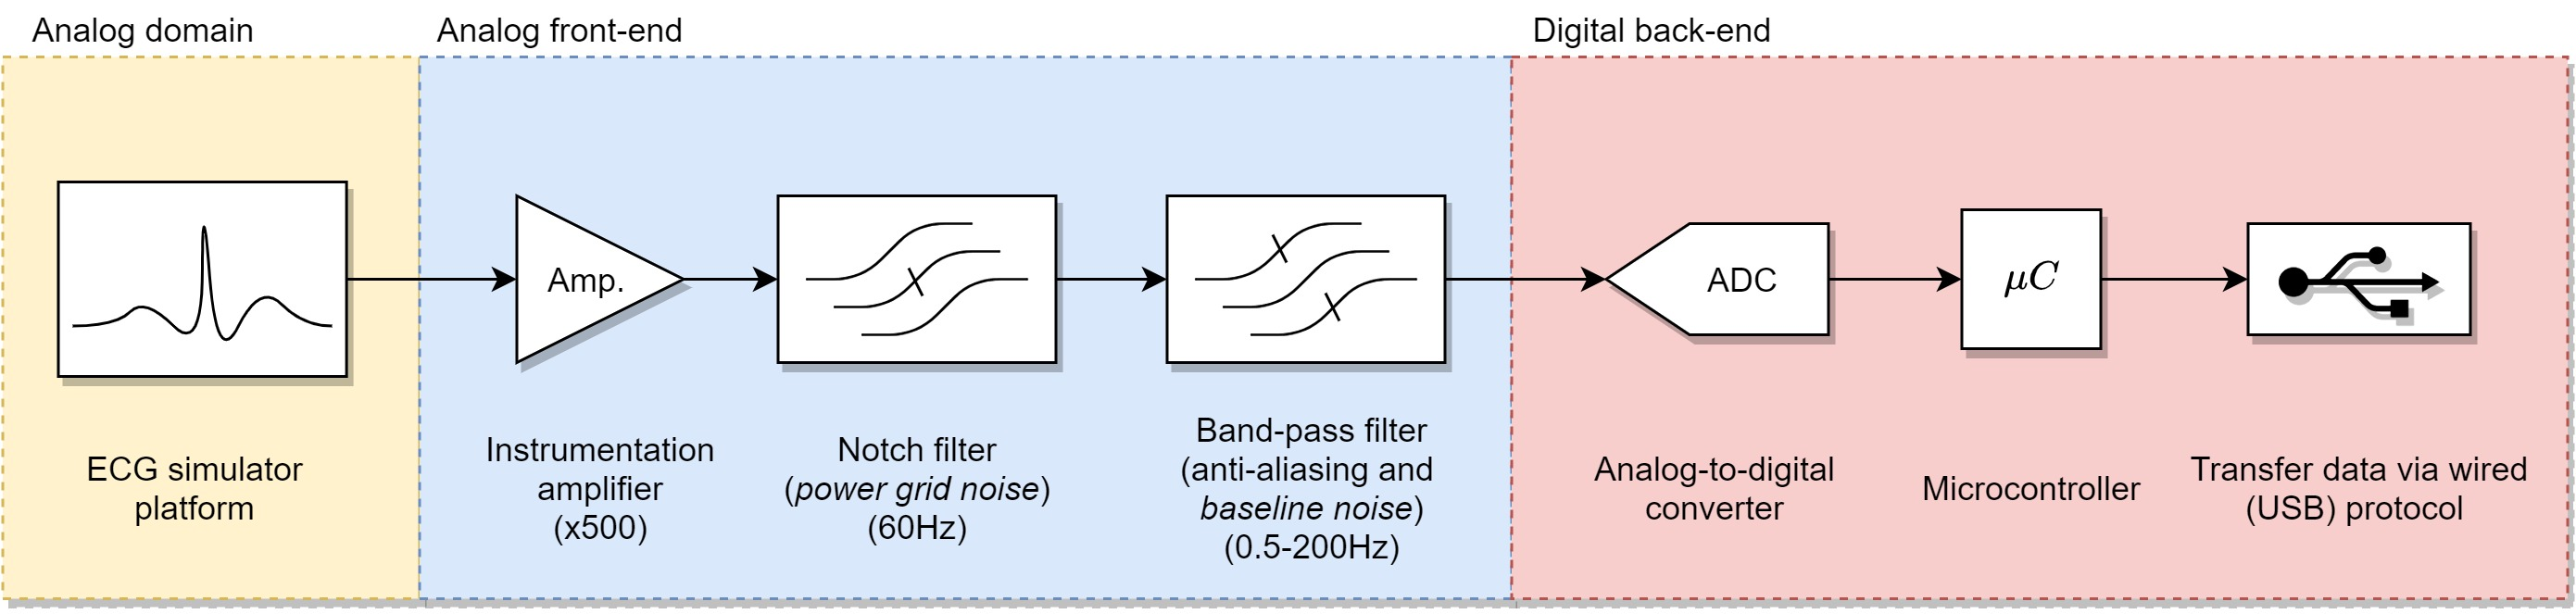
\includegraphics[width=\textwidth]{images/diagram.jpg}  
\end{center}
\end{frame}


\begin{frame}{System overview}

\begin{columns}[onlytextwidth]
    \begin{column}{0.5\textwidth}
    \begin{minipage}[c][0.5\textheight][c]{\linewidth}
        \begin{itemize}
            \item ECG simulator embedded in an ESP32 microcontroller dev-kit outputting via a built-in 8-bit DAC using the \cite{quiroz2019generation} model;
            \item Analog front-end simulated via software in LTSpice;
            \item ECG DAQ embedded in another ESP32 dev-kit with:
            \begin{itemize}
                \item Built-in 12-bit ADC;
                \item Two cores;
                \item USB interface with Python plotter client;
                \item DSP for heart rate computation and pathology analysis;
            \end{itemize}
        \end{itemize}

      \end{minipage}
      \end{column}
      
      \begin{column}{0.5\textwidth}
      \begin{minipage}[c][0.5\textheight][c]{\linewidth}
      \begin{figure}[H]
          \caption{Diagram relating the cardiac natural pacemakers to non linear variables. Source: \cite{quiroz2019generation}.}  \begin{center}
                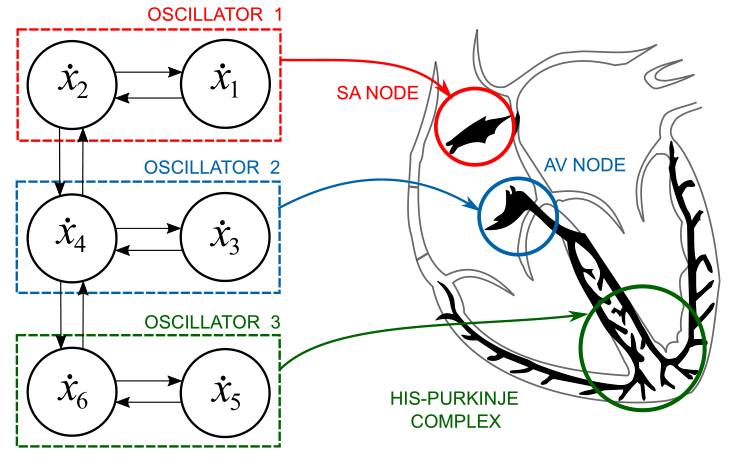
\includegraphics[width=6cm]{images/oscillators.png}  
            \end{center}
            \label{fig:2} 
            \end{figure}
        \end{minipage}
      \end{column}
\end{columns}

\end{frame}